% Report on the post-extinction-fix production runs of 2026-09-24/25 (bulge, bh, ns).
%
% Build:  cd Report/postfix && latexmk -pdf postfix_report.tex
% Figures come from the directories the analysis scripts wrote (\graphicspath below); nothing is
% copied here. The pre-fix report on the same populations is ../populations/, and is kept as is.
\documentclass[english,10pt,a4paper]{article}
\usepackage[T1]{fontenc}
\usepackage[margin=2.4cm]{geometry}
\usepackage{graphicx}
\graphicspath{{./}{../../figures/prod_20260925/}{../../figures/yield_20260925/y3/}}
\usepackage{mathtools}
\usepackage{amssymb}
\usepackage{booktabs}
\usepackage{xcolor}
\usepackage[colorlinks=true,allcolors=blue]{hyperref}
\usepackage{caption}
\usepackage[authoryear,round]{natbib}
\usepackage[section]{placeins}

\newcommand{\tE}{t_{\rm E}}
\newcommand{\piE}{\pi_{\rm E}}
\newcommand{\tetE}{\theta_{\rm E}}
\newcommand{\Ml}{M_{\rm L}}
\newcommand{\Msun}{M_\odot}
\newcommand{\Neff}{N_{\rm eff}}

\newcommand{\TODO}[1]{\textcolor{red}{\textbf{[TODO: #1]}}\typeout{TODO: #1}}

\title{The Roman--Rubin joint microlensing forecast after the extinction fix:\\
       ordinary lenses, black holes and neutron stars}
\author{Ali Salehi}
\date{\today}

\begin{document}
\maketitle

\begin{abstract}
We report the first production runs of the joint Roman\,+\,Rubin Galactic-bulge microlensing
simulation made with a corrected \citet{Cardelli1989} extinction law. Every earlier run had the law
inverted, which made Rubin's sources too bright and Roman's too faint. Three populations were
re-run with identical settings: ordinary bulge lenses, black holes (log-uniform, $3$--$1000\,\Msun$)
and neutron stars ($1.35\pm0.15\,\Msun$), each over the same 1829 sightlines. The fix halves
Rubin's yield and doubles Roman's in all three, and triples the yield of lens masses measured to
$10\%$. Per unit abundance $F$, Roman now detects $8400$ black-hole events over the decade, $1070$
of them with a $10\%$ mass; at $F_{\rm BH}=0.01$ that is $84$ events and $11$ masses. The ratio of
compact-object to ordinary yields, $\eta$, moves by less than $15\%$, as it should when the fix acts
on every population alike, and the normalisation still matches the simulator's own optical depth to
$0.1\%$. On the events both surveys characterise, Rubin now adds essentially nothing to Roman's
precision (median gain $<0.3\%$, was $\sim\!35\%$); its contribution is the $70\%$ of events outside
Roman's footprint and the short events that peak deep inside Roman's season gaps, where the
gap-filling gain survives at full strength but no longer dominates the pooled numbers. Against
\citet{SajadianSahu2023}, the fix closes most of the astrometric shortfall but little of the
parallax one, so the extinction law was not its main cause. All counts are Monte Carlo errors only;
full-scan yields also carry the model's shallow latitude gradient, still to be re-measured on these
runs.
\end{abstract}

% -------------------------------------------------------------------------------------------------
\section{Simulation and runs}

The simulator, its Fisher matrices and the event-rate weight are unchanged from the compact-object
report (\texttt{Report/populations/}), whose Section~1 describes them. In brief: source stars and
lenses are drawn along each sightline from Besan\c{c}on \citep{Robin2003}/CMD population models
with three-dimensional dust extinction, per-band light curves are generated against the real Rubin
visit list and the published Roman GBTDS cadence \citep{ROTAC2025}, a Monte Carlo detection test
with a fixed $\Delta\chi^2\ge500$ is applied, and every detected event is characterised three
times -- by Rubin alone, by Roman alone, and jointly -- through independent Fisher matrices.

What is new is the photometry. Every run before 2026-09-22 evaluated the \citet{Cardelli1989}
reddening law at $1/\lambda$ instead of $\lambda$, which inverted it: $A_u/A_V$ came out as $0.07$
instead of $1.69$, and $A_{F146}/A_V$ as $0.75$ instead of $0.20$ (Deviations~52--53). Rubin's
sources were therefore far too bright and Roman's too faint. The three runs reported here are the
first with the corrected law. They are otherwise identical to the pre-fix runs -- same flags
(\verb|--events 300 --lenses 50| \verb|--stride-roman 5 --pair-satellite|), same seed, same
1829-sightline grid -- so their differences from the earlier runs are the fix and nothing else.
All three were made at commit \texttt{a5028fe} (Table~\ref{tab:runs}).

\begin{table}[h]
\centering
\caption{Run configuration and outcome. ``Detected draws'' is a \emph{Monte Carlo sample size},
set by the stopping rule (at least $50$ detections per sightline), not a forecast: every lens is
drawn from the population under test, i.e.\ $F=1$ implicitly; Section~\ref{sec:yield} converts
it to a yield. ``Barren'' sightlines drew stars but characterised nothing, and carry no weight.
The weightable draws are the ones every number in this report is computed from; the bracket gives
the ratio to the pre-fix run, a direct measure of the extra cost of the fix (fainter Rubin sources
mean more draws per detection).}
\label{tab:runs}
\small
\begin{tabular}{lrrr}
\toprule
 & ordinary lenses & black holes & neutron stars \\
\midrule
mass function         & Kroupa + remnants & log-uniform & Gaussian \\
mass range [$\Msun$]  & ---               & $3$--$1000$ & $1.35\pm0.15$ \\
sightlines aggregated & 1612 & 1612 & 1612 \\
\quad no coverage / barren & 140 / 77 & 140 / 77 & 140 / 77 \\
\quad stopped on the draw cap & 115 & 79 & 86 \\
rows written          & 12\,222\,487 & 6\,486\,605 & 8\,388\,536 \\
weightable draws      & 8\,372\,487 & 2\,636\,605\ ($3.2\times$) & 4\,538\,536\ ($3.9\times$) \\
detected draws (MC)   & 85\,061 & 101\,515 & 93\,185 \\
\quad Rubin + joint     & 73\,517 & 77\,683 & 75\,027 \\
\quad Roman + joint     & 9\,452  & 18\,007 & 14\,441 \\
\quad both + joint      & 2\,016  & 5\,764  & 3\,606 \\
$\Neff$ (weighted)    & --- & 210\,993 & 478\,123 \\
\bottomrule
\end{tabular}
\end{table}

The three indented detection rows split the detections by which survey clears the bar on its own:
Rubin but not Roman, Roman but not Rubin, or both (a handful clear it only jointly). The ordinary-lens run is used here only for the yields and for $\eta$
(Section~\ref{sec:yield}); the figures of Sections~\ref{sec:synergy}--\ref{sec:where} cover the
two compact-object populations, as in the pre-fix report.

\paragraph{Weighting.} The Monte Carlo draws the lens distance in proportion to the event rate but
the lens mass from the number density and the velocities from plain Gaussians, so it lacks the
rate's $\sqrt{\Ml}\,v_t$ factor. Every pooled fraction, median or ratio therefore carries the
per-event weight $W \propto w_{\rm area}\,N_\star/n_{\rm sim}\,\sqrt{\Ml}\,v_t\,Z(D_s)$ and is
quoted with the \citet{Kish1965} effective sample size $\Neff = (\sum w)^2/\sum w^2$.

% -------------------------------------------------------------------------------------------------
\section{What the extinction fix changed}
\label{sec:fix}

Because the runs differ only in the extinction law, the cleanest measure of the fix is the yield
per unit abundance $N_1$ (Section~\ref{sec:yield}) before and after, selection by selection
(Table~\ref{tab:fix}). $N_1$ is used rather than the raw detected counts because those are sample
sizes, fixed by the stopping rule, and would hide the change.

\begin{table}[h]
\centering
\caption{Yield per unit abundance, post-fix over pre-fix, whole scan, per-object convention.
Pre-fix: the runs of 2026-09-17 (compact objects) and 2026-09-06 (ordinary lenses). Every ratio
is at least $3\sigma$ from unity in Monte Carlo error except the ordinary-lens
$\sigma(\Ml)/\Ml<1\%$ row ($1.4\sigma$). Source: \texttt{figures/yield\_20260925/compare\_20260922.md}.}
\label{tab:fix}
\begin{tabular}{lrrr}
\toprule
selection & ordinary lenses & black holes & neutron stars \\
\midrule
either survey detects        & 0.65 & 0.66 & 0.67 \\
Rubin detects                & 0.50 & 0.55 & 0.53 \\
Roman detects                & 1.99 & 1.71 & 2.06 \\
both detect                  & 0.79 & 0.72 & 0.74 \\
Rubin only                   & 0.49 & 0.54 & 0.52 \\
Roman only                   & 2.49 & 2.68 & 2.81 \\
Roman, $\sigma(\Ml)/\Ml<10\%$ & 3.02 & 2.83 & 3.23 \\
joint, $\sigma(\Ml)/\Ml<10\%$ & 2.67 & 1.85 & 2.68 \\
\midrule
Rubin only, inside Roman's footprint & 0.50 & 0.17 & 0.43 \\
\bottomrule
\end{tabular}
\end{table}

The pattern is the one the bug predicted, and it holds in all three populations. Rubin's yield
halves, because its sources now carry the optical extinction they should: at the median
$A_V\approx3.8$ of these sightlines the $r$-band source is several magnitudes fainter than before.
Roman's roughly doubles, because in F146 the extinction fell by a factor $\sim\!4$. The total
falls by a third, since Rubin dominated it. The mass-precision yields gain the most, a factor
$\sim\!3$, because a brighter Roman source improves both the photometric parallax and the
astrometric $\tetE$ that the mass needs.

Two consequences matter for how the earlier results are read. First, Rubin no longer dominates
inside Roman's footprint: there, Rubin-only black-hole events fall to $0.17$ of their pre-fix
yield, to $66$ per unit $F$, against $6653$ Roman-only. Second, the survey-share and joint-gain
numbers of the pre-fix report (its Table~2) were biased in Rubin's favour, as that report
warned; the revised ones are in Section~\ref{sec:synergy}.

% -------------------------------------------------------------------------------------------------
\section{What each survey contributes}
\label{sec:synergy}

\begin{figure}[h]
\centering
\includegraphics[width=\textwidth]{p6_synergy.png}
\caption{(a) Weighted share of detected events found by each survey. (b) Median ratio of the
joint to the single-survey error, \emph{restricted to events that both surveys characterised
independently}; pooled over all characterised events the joint fit is the Rubin fit for most of
them and the ratio would be $1$ by construction.}
\label{fig:synergy}
\end{figure}

Table~\ref{tab:synergy} gives the numbers, beside the pre-fix ones. Roman's share of the
detections quadruples, from $5$--$6\%$ to $21$--$26\%$, although its footprint is still only
$\sim\!2\%$ of the scanned sky: Roman now finds more than a fifth of all events from a fiftieth of
the area.

\begin{table}[h]
\centering
\caption{Detection provenance and the joint-fit gain, post-fix (pre-fix in brackets, from the
compact-object report). Detection shares are weighted over all detections, whole scan. The
$\sigma$ ratios are weighted medians over events characterised independently by \emph{both}
surveys ($23\,961$ black-hole and $18\,895$ neutron-star events, against $15\,849$ and $12\,569$
before); below unity means the joint fit is better. Source:
\texttt{figures/prod\_20260925/p6\_synergy\_resolution.log}.}
\label{tab:synergy}
\begin{tabular}{lrrrr}
\toprule
 & \multicolumn{2}{c}{black holes} & \multicolumn{2}{c}{neutron stars} \\
\cmidrule(lr){2-3}\cmidrule(lr){4-5}
 & vs.\ Rubin & vs.\ Roman & vs.\ Rubin & vs.\ Roman \\
\midrule
detected by Rubin only [\%] & \multicolumn{2}{c}{72.9 (89.4)} & \multicolumn{2}{c}{69.6 (90.0)} \\
detected by Roman only [\%] & \multicolumn{2}{c}{21.5 (5.3)}  & \multicolumn{2}{c}{26.3 (6.3)} \\
detected by both [\%]       & \multicolumn{2}{c}{5.6 (5.2)}   & \multicolumn{2}{c}{3.9 (3.6)} \\
\midrule
median $\sigma(\tE)$ ratio    & 0.022 (0.165) & 0.997 (0.733) & 0.008 (0.116) & 0.999 (0.742) \\
median $\sigma(\piE)$ ratio   & 0.010 (0.108) & 0.998 (0.826) & 0.008 (0.114) & 0.999 (0.798) \\
median $\sigma(\tetE)$ ratio  & 0.041 (0.187) & 0.999 (0.979) & 0.035 (0.152) & 0.999 (0.975) \\
\bottomrule
\end{tabular}
\end{table}

The joint-fit gain changes more than any other number in this report, and in a way that reverses
one of the pre-fix conclusions. Before the fix, Rubin's decade-long baseline improved Roman's
timescale by $\sim\!1.35\times$ and its parallax by $\sim\!1.2\times$. After it, on the events both
surveys characterise, Rubin adds nothing measurable to Roman: the median joint/Roman ratio is
$0.997$--$0.999$ for every parameter and both populations, and panel (b) shows it flat at unity
across four decades of $\tE$, including the multi-year events where Rubin's baseline should matter
most. In the other direction the gain grew by an order of magnitude, to a factor $25$--$125$
over Rubin alone.

Both follow from where these events are. The events both surveys characterise lie inside Roman's
footprint, at low latitude, where the median $A_V\approx3.8$ now costs Rubin's $r$-band source
several magnitudes and Roman's F146 source only $\sim\!0.7$. Rubin's per-point precision on these
sources has fallen far below Roman's, while Roman's $\sim\!50\,000$ epochs over the ten seasons
already span most of the baseline Rubin was contributing. The pre-fix gain was an artefact of
sources that were too bright for Rubin and too faint for Roman. The joint science case inside the
footprint is therefore Roman's; Rubin's contribution is the $70\%$ of events it finds \emph{outside}
the footprint, and the Rubin-only detections it makes of events that peak outside Roman's
mission.

\paragraph{Gap filling survives, but only deep inside the gaps.} The compact-object report did not
cover the gap-filling result of the whitepaper -- Rubin recovering short events that peak between
Roman's seasons -- but it is the result the fix moves most, so it is recorded here from the
ordinary-lens run (\texttt{figures/wp\_20260926/}). Pooled over every footprint event with
$10\le\tE<30$\,d peaking in a gap, the weighted median $\sigma_{\rm joint}(\tE)/\sigma_{\rm Roman}(\tE)$
is now $0.973$ ($\Neff=670$), against $0.261$ before the fix. Deep in a gap the effect is intact:
for peaks more than $30$\,d from the nearest season edge the median is $0.44$, and beyond $45$\,d
it is $0.077$ ($\Neff=62$; $0.007$ before). With Roman's sources now as bright as they should be,
Roman's wing coverage settles any event peaking near a season edge, and Rubin is decisive only for
events that begin and end inside a gap. The joint fit characterises $2.0\%$ (weighted) of in-gap
footprint detections that Roman alone does not.

% -------------------------------------------------------------------------------------------------
\section{Fisher forecast precision}

\begin{figure}[h]
\centering
\includegraphics[width=\textwidth,trim=0 14 508 0,clip]{p7_precision.png}
\caption{Weighted cumulative distribution of the fractional parameter error, per survey and
population. \textbf{Each curve is over its own characterised set}: Roman characterises only inside
its footprint, while the joint curve also contains every Rubin-only event, so a Roman curve lying
above the joint one is a difference of samples, not a violation of
$\sigma_{\rm joint}\le\sigma_{\rm single}$. Event-rate weighted; $\Neff=210\,993$ (black holes)
and $478\,123$ (neutron stars); commit \texttt{a5028fe}. Dotted: the $10\%$ criterion.}
\label{fig:precision}
\end{figure}

\begin{table}[h]
\centering
\caption{Weighted fraction of characterised events measured to better than $10\%$, post-fix
(pre-fix in brackets). Read down a column, not across: each entry has its own denominator
(Fig.~\ref{fig:precision}). Source: \texttt{figures/prod\_20260925/p7\_forecast\_figures.log}.}
\label{tab:tenpercent}
\small
\begin{tabular}{lrrr}
\toprule
 & joint [\%] & Rubin [\%] & Roman [\%] \\
\midrule
\multicolumn{4}{l}{\emph{black holes}} \\
$\tE$   & 18.7 (19.8) & 11.7 (17.7) & 23.6 (18.6) \\
$\piE$  &  5.3 (3.1)  &  1.5 (2.1)  & 12.9 (7.7)  \\
$\tetE$ & 48.8 (43.9) & 37.5 (41.1) & 97.0 (81.4) \\
$\Ml$   &  4.2 (1.5)  &  0.3 (0.4)  & 12.6 (7.1)  \\
\midrule
\multicolumn{4}{l}{\emph{neutron stars}} \\
$\tE$   & 10.0 (7.7)  &  4.5 (6.1)  & 16.0 (10.5) \\
$\piE$  &  2.4 (1.5)  &  0.8 (1.1)  &  4.6 (2.9)  \\
$\tetE$ & 22.1 (6.0)  &  0.4 (0.4)  & 67.2 (42.3) \\
$\Ml$   &  1.4 (0.3)  &  0.0 (0.0)  &  3.7 (1.9)  \\
\bottomrule
\end{tabular}
\end{table}

Every Roman entry improves and every Rubin entry but one worsens, the direct image of
Table~\ref{tab:fix}. Roman now measures $\tetE$ to $10\%$ for $97\%$ of the black-hole events it
characterises and $67\%$ of the neutron-star ones (from $81$ and $42\%$), and the lens mass for
$12.6\%$ and $3.7\%$ (from $7.1$ and $1.9\%$). The joint column rises less than Roman's for most
entries, because it is dominated by Rubin-only events outside the footprint, whose precision fell;
for the neutron-star $\tetE$ it nonetheless rises from $6$ to $22\%$, because Roman characterises a
larger share of all events than before. The lens mass remains the hardest quantity, being the
ratio of $\tetE$ to $\piE$ and limited by $\piE$, which even Roman measures to $10\%$ for only
$13\%$ of black-hole and $5\%$ of neutron-star events.

\begin{figure}[h]
\centering
\includegraphics[width=\textwidth]{p7_precision_te.png}
\caption{Median fractional error against the event timescale. Rubin's $\sim\!3$-day cadence
under-resolves short events; Roman's $72$-day seasons cannot contain long ones, which is where
Rubin's decade of coverage matters.}
\label{fig:precision_te}
\end{figure}

% -------------------------------------------------------------------------------------------------
\section{Astrometry, satellite parallax and image resolution}

\begin{figure}[h]
\centering
\includegraphics[width=\textwidth]{p6_astrometry.png}
\caption{(a) Weighted distribution of the maximum centroid shift reached by each event. (b) The
blend-diluted shift against lens mass, with the weighted interquartile band; the dotted line is
Roman's $1.1$\,mas per-exposure astrometric floor.}
\label{fig:astrometry}
\end{figure}

\begin{table}[h]
\centering
\caption{Astrometric shift, satellite parallax and image resolvability, post-fix (pre-fix in
brackets). The resolution probability is the weighted fraction of that survey's detections with at
least three epochs at which both images are detectable and separated by more than the bar
($\mathcal{D}\sigma_a$ or the PSF FWHM). Source: \texttt{p6\_synergy\_resolution.log}.}
\label{tab:ast}
\begin{tabular}{lrr}
\toprule
 & black holes & neutron stars \\
\midrule
median max.\ centroid shift [mas]      & 3.60 (3.61)  & 0.264 (0.265) \\
95th percentile [mas]                  & 9.70 (9.75)  & 0.604 (0.610) \\
fraction above $1.1$\,mas floor [\%]   & 90.4 (90.2)  & 0.58 (0.57) \\
\midrule
satellite parallax, median gain        & 1.000 (1.000) & 1.000 (1.000) \\
\quad fraction gaining $>1.1\times$ [\%] & 0.001 (0.003) & 0.151 (0.200) \\
\quad fraction gaining $>2\times$ [\%]   & 0.000 (0.000) & 0.040 (0.064) \\
\midrule
$P(\text{resolve})$ Rubin, $\mathcal{D}=5$ [\%]  & 5.45 (16.71)  & 0.0002 (0.0015) \\
$P(\text{resolve})$ Roman, $\mathcal{D}=5$ [\%]  & 65.5 (41.6)   & 14.9 (6.13) \\
$P(\text{resolve})$ Roman, $\mathcal{D}=20$ [\%] & 30.9 (14.0)   & 0.35 (0.171) \\
$P(\text{resolve})$ Roman, PSF FWHM [\%]         & 0.68 (0.875)  & 0.0011 (0.0001) \\
\bottomrule
\end{tabular}
\end{table}

\paragraph{The centroid shift is unchanged, as it must be.} The shift
$\delta\theta = \tetE u/(u^2+2)$ is geometry: it depends on the lens and the trajectory, not on the
source's brightness. The fix changes which events are detected, not their geometry, so the
distributions agree with the pre-fix ones to within $1\%$ -- black holes still cross Roman's
per-exposure floor for $90\%$ of detections, neutron stars for $0.6\%$. This is a useful control:
a change here would have meant the fix leaked into something it should not touch.

\paragraph{Satellite parallax remains worthless for these populations.} The median gain from L2
is exactly $1$ and fewer than $0.2\%$ of events gain $10\%$; the fix does not change the geometry
that makes L2's $0.01$\,au baseline negligible for events lasting months to years.

\paragraph{Image resolution now favours Roman even more.} Resolving the images needs \emph{both}
to be detectable, and the minor image is faint, so the probability tracks source brightness.
Roman's rises (black holes $41.6\to65.5\%$ at $\mathcal{D}=5$, $14.0\to30.9\%$ at
$\mathcal{D}=20$) and Rubin's falls ($16.7\to5.5\%$). The PSF criterion moves little and the other
way for black holes ($0.88\to0.68\%$), because the separation must there exceed the $105$\,mas
FWHM, which only the nearest, heaviest lenses reach; the brightness gain barely enters. The
dependence on the chosen criterion -- two orders of magnitude between $\mathcal{D}=5$ and the PSF
bar -- still outweighs every other effect, and is why all three are reported.

\begin{figure}[h]
\centering
\includegraphics[width=\textwidth]{p6_parallax.png}
\caption{Survival function of the gain from placing Roman at L2 rather than at Earth, for the
parallax (a) and the lens mass (b); the same event is characterised twice, differing only in the
observer's position. Logarithmic vertical axis.}
\label{fig:parallax}
\end{figure}

\begin{figure}[h]
\centering
\includegraphics[width=\textwidth,trim=0 14 299 0,clip]{p6_resolution.png}
\caption{(a) Probability that the two lensing-induced images are resolvable, for three resolution
criteria, following \citet{SajadianMakler2026}: at least three epochs with both images detectable
and separated by more than the bar. (b) The same at the most permissive criterion, against lens
mass. Event-rate weighted, same $\Neff$ as Fig.~\ref{fig:precision}; $\mathcal{D}=5$ and $20$ are
$\mathcal{D}\sigma_a$, PSF is the filter's FWHM.}
\label{fig:resolution}
\end{figure}

% -------------------------------------------------------------------------------------------------
\section{Where the measurable lenses are}
\label{sec:where}

\begin{figure}[h]
\centering
\includegraphics[width=\textwidth]{p7_mass_distance.png}
\caption{Weighted fraction of detected events whose lens mass is measured to better than $10\%$,
in the mass--distance plane.}
\label{fig:massdist}
\end{figure}

Across all detections, the joint fit now measures the lens mass to $10\%$ for $4.16\%$ of
black-hole events (median lens distance $5.53$\,kpc) and $1.36\%$ of neutron-star events (median
$4.13$\,kpc), against $1.50\%$ and $0.34\%$ before the fix. The measurable lenses are still the
near, heavy ones that $\tetE=\sqrt{\kappa\Ml\pi_{\rm rel}}$ favours, but less exclusively: the median
distance of a measured lens moved outward by $\sim\!0.4$\,kpc in both populations, because a
brighter Roman source lets a smaller $\tetE$ be measured.

\begin{figure}[h]
\centering
\includegraphics[width=\textwidth]{p7_sky.png}
\caption{(a) Relative weighted event yield across the scanned region, black-hole run.
(b) Weighted fraction of detections with $\sigma(\tE)/\tE<0.1$ from the joint fit.}
\label{fig:sky}
\end{figure}

% -------------------------------------------------------------------------------------------------
\section{Absolute event yields}
\label{sec:yield}

The derivation, the choice of abundance grid and the recipe are in the compact-object report
(\S8); only the results change. Each draw carries the event rate it stands for, and the expected
number of events whose peak falls in the ten-year window is $N(F) = F\,N_1$, exactly linear in the
abundance $F$ -- the fraction of the Galaxy's stellar mass in the population. $N_1$ is the yield
at $F=1$; for the ordinary-lens run $F=1$ by definition, so its $N_1$ are yields as they stand.
Two counting conventions are given: per resolved object (the simulator keeps a blended source with
probability equal to its blend fraction, as in \citealt{SajadianSahu2023} and
\citealt{SajadianMakler2026}) and all stars (that thinning undone); they differ by $1$--$8\%$ here.

\paragraph{Normalisation.} The optical depth rebuilt from the rate constants,
$\tau = (\pi/2u_{0,\max})\langle\gamma\,\tE\rangle$, over the one the C++ computes independently
per sightline, pooled over all sightlines: $1.001$ (ordinary lenses), $1.001$ (black holes) and
$1.000$ (neutron stars). The fix does not touch the rate, only which events are detected, and the
check confirms the normalisation survived the re-run.

\begin{table}[h]
\centering
\caption{Yield per unit abundance $N_1$: expected events over the ten-year window at $F=1$,
inside Roman's $1.47\,\mathrm{deg}^2$ footprint unless stated, per-object convention (all-stars
convention in brackets for the two headline rows). Multiply by $F$ for a yield. Errors are Monte
Carlo only. $\eta = N_1/N_1^{\rm ordinary}$ for the same selection: the fraction of all events a
population supplies per unit mass fraction. Source: \texttt{figures/yield\_20260925/y3/}.}
\label{tab:n1}
\small
\begin{tabular}{lrrr}
\toprule
selection & black holes & neutron stars & ordinary lenses \\
\midrule
either survey detects         & $8477\pm91$  & $62\,400\pm680$ & $89\,700\pm1400$ \\
Roman detects                 & $8398\pm91$\ (8972) & $57\,900\pm650$\ (60\,600) & $81\,900\pm1400$\ (86\,800) \\
Rubin detects                 & $1812\pm40$  & $11\,560\pm280$ & $16\,830\pm640$ \\
both detect                   & $1746\pm40$  & $7520\pm220$    & $9490\pm480$ \\
Roman only                    & $6653\pm81$  & $50\,400\pm610$ & $72\,400\pm1300$ \\
Rubin only                    & $65.7\pm5.3$ & $4040\pm180$    & $7340\pm430$ \\
Roman, $\sigma(\Ml)/\Ml<1\%$  & $59.8\pm5.9$ & $40.5\pm4.5$    & $11.7\pm3.9$ \\
Roman, $\sigma(\Ml)/\Ml<5\%$  & $589\pm22$   & $960\pm50$      & $1010\pm240$ \\
Roman, $\sigma(\Ml)/\Ml<10\%$ & $1068\pm31$  & $2286\pm90$     & $1930\pm260$ \\
joint, $\sigma(\Ml)/\Ml<10\%$ & $1216\pm33$  & $2599\pm95$     & $2120\pm270$ \\
\midrule
Rubin detects, full $59\,\mathrm{deg}^2$ & $24\,340\pm220$\ (24\,920) & $141\,100\pm1300$\ (144\,100) & $174\,900\pm2200$ \\
either survey, full scan & $31\,010\pm230$ & $191\,900\pm1500$ & $247\,800\pm2500$ \\
\midrule
$\eta$, Roman detects             & 0.103 & 0.708 & \\
$\eta$, Rubin detects (full scan) & 0.139 & 0.806 & \\
$\eta$, either survey (full scan) & 0.125 & 0.774 & \\
\bottomrule
\end{tabular}
\end{table}

\begin{figure}[h]
\centering
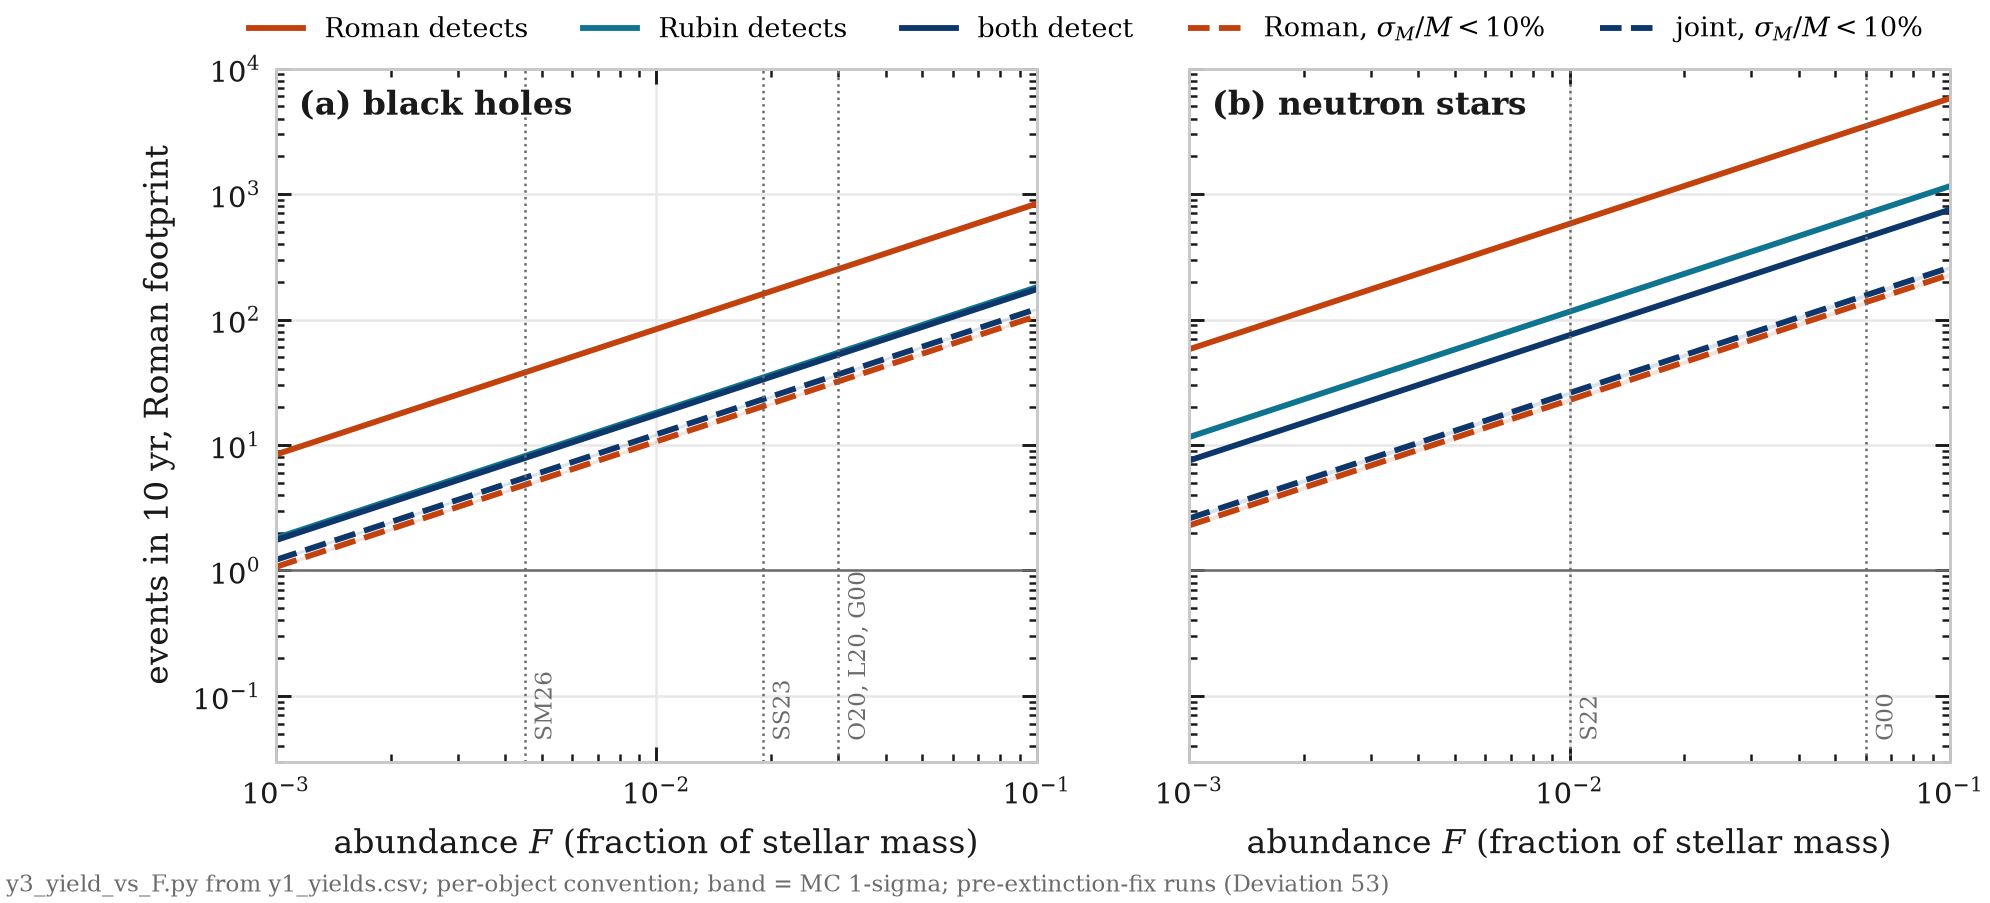
\includegraphics[width=\textwidth]{y3_yield_vs_F.png}
\caption{Expected events over the ten-year window inside Roman's footprint against the assumed
abundance, $N(F)=F\,N_1$; shaded bands are the Monte Carlo $1\sigma$. Dotted verticals mark the
literature abundances: SM26 \citet{SajadianMakler2026}; SS23 \citet{SajadianSahu2023}, their $F_1$;
O20, L20, G00 \citet{Olejak2020}, \citet{Lam2020}, \citet{Gould2000}; S22 \citet{Sweeney2022}, for
neutron stars and black holes together. The horizontal line is one event. Black holes over
$3$--$1000\,\Msun$ as simulated; per-object convention.}
\label{fig:yieldF}
\end{figure}

\paragraph{Reading the numbers.} Roman now detects black holes at $\sim\!84$ events per per cent
of stellar mass (was $49$), so the literature range $F_{\rm BH}=0.005$--$0.03$ gives $42$--$250$
events over the decade, of which $5$--$32$ have their mass measured to $10\%$ by Roman alone. For
neutron stars, $F_{\rm NS}=0.005$--$0.06$ gives $290$--$3500$ Roman detections and $11$--$140$
masses to $10\%$. To expect one black hole with a $10\%$ mass, $F_{\rm BH}\gtrsim10^{-3}$ now
suffices (was $\sim\!0.003$).

$\eta$ barely moves: $0.103$ against $0.119$ before the fix for Roman black-hole detections,
$0.708$ against $0.683$ for neutron stars. That is expected, and is the strongest internal check
of this section: the fix changes which sources are bright enough, which acts on every lens
population alike, and so cancels in a ratio of populations. The mass-precision rows do \emph{not}
give a stable $\eta$ -- for $\sigma(\Ml)/\Ml<1\%$ black holes outnumber ordinary lenses per unit
$F$ ($59.8$ against $11.7$), because only a heavy lens gives a $\tetE$ large enough -- and the
ordinary-lens entries there rest on $32$--$1089$ Monte Carlo events, so their $\eta$ is not quoted.

\paragraph{Which Roman detections saw the peak.} With $\sim\!50\,000$ exposures, Roman can pass
$\Delta\chi^2\ge500$ on the slow wing of an event whose peak it never observed, so part of its
doubled yield could in principle be wing detections. Table~\ref{tab:peak} splits the Roman-detected
yield by where the peak falls; the numbers come from
\texttt{y5\_roman\_peak\_coverage.py}.

\begin{table}[h]
\centering
\caption{Fraction of the Roman-detected yield (whole scan, per object, $F=1$) by peak position.
The first three rows partition the total; the last counts events with no Roman epoch within
$\pm2\tE$ of $t_0$. Source: \texttt{figures/yield\_20260925/y5\_peak\_coverage.md}.}
\label{tab:peak}
\begin{tabular}{lrrr}
\toprule
 & black holes & neutron stars & ordinary lenses \\
\midrule
peak in a Roman season            & 0.225 & 0.402 & 0.542 \\
peak in a gap between seasons     & 0.320 & 0.467 & 0.373 \\
peak outside Roman's mission      & 0.455 & 0.131 & 0.085 \\
\midrule
no Roman epoch within $\pm2\tE$   & 0.029 & 0.039 & 0.044 \\
\bottomrule
\end{tabular}
\end{table}

Nearly half of Roman's black-hole yield peaks outside its mission, but only $3\%$ has no Roman epoch
within $\pm2\tE$: a black-hole event lasts hundreds of days, so Roman observes the magnified part
of most events that peak after its last season. Across all three populations only $3$--$4\%$ of the
Roman yield is a pure wing detection. The Roman rows of Table~\ref{tab:n1} therefore describe events
Roman genuinely observed while magnified; a peak-coverage requirement would lower them by at most
$4.4\%$.

% -------------------------------------------------------------------------------------------------
\section{Comparison with \texorpdfstring{\citet{SajadianSahu2023}}{Sajadian \& Sahu (2023)}}

The pre-fix report aligned the two calculations (their $F_1=0.019$ is our $F$; their
$\mathrm{d}N/\mathrm{d}M\propto M^{-1}$ row matches our log-uniform function; we re-weight our
draws to $3$--$50\,\Msun$ against their $2$--$50$) and found that we detect $2.3\times$ more black
holes per unit area and season than they do but characterise a smaller fraction, with the deficit
concentrated on the parallax. It listed the extinction law as the first candidate for the
deficit. Both comparisons are repeated here on the corrected run.

\paragraph{Detections.} Re-weighted to $3$--$50\,\Msun$ at $F=0.019$, Roman detects $464$ black
holes in its footprint over ten seasons (\texttt{figures/yield\_20260925/bh/y1\_yields.md}),
$31.5$ per deg$^2$ per season against their $7.2$ -- a factor $4.4$, up from $2.3$. The excess was
already attributed to the survey design (the final GBTDS fills the $2.3$-year gap their forecast
was built around, \citealt{ROTAC2025}) and to their stricter detection cut; the fix doubles Roman's
detections and so doubles it.

\paragraph{Characterisation.} On their denominator (fraction of Roman detections) and the
matched mass range, at the $10\%$ threshold (\texttt{figures/y2\_20260925/y2\_ss23.md}):

\begin{center}
\begin{tabular}{lrrrr}
\toprule
 & SS23 [\%] & pre-fix [\%] & post-fix [\%] & post-fix / SS23 \\
\midrule
$\sigma(\tetE)/\tetE < 10\%$ & 99.2 & 68.6 & 88.8 & 0.90 \\
$\sigma(\tE)/\tE < 10\%$     & 67.0 & 21.7 & 26.0 & 0.39 \\
$\sigma(\piE)/\piE < 10\%$   & 30.0 &  7.4 & 10.0 & 0.33 \\
$\sigma(\Ml)/\Ml < 10\%$     & 29.8 &  6.2 &  9.3 & 0.31 \\
\bottomrule
\end{tabular}
\end{center}

The fix closes most of the astrometric gap -- $\tetE$ goes from $0.69$ to $0.90$ of their value,
as brighter F146 sources should -- but only a small part of the photometric one: $\tE$ and $\piE$
remain at a third of theirs. The extinction law was therefore not the main cause of the parallax
shortfall, and the open item on it stays open with its remaining candidates: whether the
astrometric and photometric $\piE$ information are combined, and the long parallax baseline their
hand-added gap observations provide. Their detections are counted at a higher bar
($\Delta\chi^2>800$ plus three $4\sigma$ points), which removes marginal events that are the
hardest to characterise and so raises their fractions; how much of the remaining factor $3$ that
accounts for has not been measured.

% -------------------------------------------------------------------------------------------------
\section{Caveats}

\begin{itemize}
\item \textbf{The populations are run separately and must not be pooled.} The event-rate weight
      contains $\sqrt{\Ml}$ of the mass function actually sampled; black-hole and neutron-star
      yields add as $F_{\rm BH}N_{1,\rm BH}+F_{\rm NS}N_{1,\rm NS}$, but their draws must not share
      a weighted statistic.
\item \textbf{The log-uniform black-hole mass function is an assumption}, taken as the truth
      rather than as an importance-sampling device.
\item \textbf{Absolute yields scale with an assumed abundance $F$}, uncertain by an order of
      magnitude; $N_1$ is given so that any $F$ can be used.
\item \textbf{The model's latitude gradient is too shallow} against OGLE-IV \citep{Mroz2019}:
      measured on the pre-fix data it over-produces events by $\sim\!40\%$ at $b=-5^\circ$ and
      under-produces them near the plane. That comparison used an $I<21$ cut that the extinction
      law acts on directly, so it must be re-measured on these runs; until then full-scan yields
      carry a systematic of a few tens of per cent. Footprint yields are less affected.
\item \textbf{Roman's parallax precision is still $\sim\!3\times$ worse than
      \citet{SajadianSahu2023}}, with the extinction law now ruled out as the main cause.
\item \textbf{One detection-test anomaly.} The ordinary-lens run records one event (of $85\,061$)
      where a single-survey test passed and the joint test did not, which the construction of the
      tests should forbid. The detection flag is made monotone downstream, so no table is wrong;
      the cause is open.
\item \textbf{Draw-capped sightlines.} $79$--$115$ sightlines per run stopped at the draw cap with
      fewer than $50$ detections; their Monte Carlo error is larger than requested, and is
      included in the quoted errors.
\item \textbf{Rubin's astrometric error model is the weakest input}: a $10$\,mas per-visit floor
      against published estimates of $3$--$7$\,mas.
\end{itemize}

% -------------------------------------------------------------------------------------------------
\section*{Reproducing this report}

\begin{verbatim}
runs/yields_20260925.sh                    # y1 for bh, ns, bulge in turn, then y3
.roman/bin/python analysis/y4_compare_yields.py \
    figures/yield_prefix_20260922/y1_yields.csv figures/yield_20260925/y1_yields.csv \
    -o figures/yield_20260925/compare_20260922.md
.roman/bin/python analysis/y5_roman_peak_coverage.py --run bh=runs/prod_bh_20260924 \
    --run ns=runs/prod_ns_20260924 --run bulge=runs/prod_bulge_20260924 \
    -o figures/yield_20260925/y5_peak_coverage.md
.roman/bin/python analysis/y2_ss23_compare.py --run runs/prod_bh_20260924 \
    -o figures/y2_20260925/y2_ss23
figures/prod_20260925/run_p67.sh           # p6 and p7 on bh + ns
cd Report/postfix && latexmk -pdf postfix_report.tex
\end{verbatim}

\bibliographystyle{plainnat}
\bibliography{../refs}

\end{document}
